%!TEX root = pdl.tex

\section{Organisation du projet}
\subsection{Structure d’organisation}
L'équipe est composée de quatre membres.
\begin{itemize}
	\item Badre Baba, architecte ;
	\item Geoffroy Carrier, développeur ;
	\item Jean-Christophe Saad-Dupuy, chef de projet ;
	\item Scheer Mickael, responsable qualité.
\end{itemize}

%\subsection{Interfaces externes}
\subsection{Rôles et responsabilités}
\begin{figure}[thbp]
	\centering
		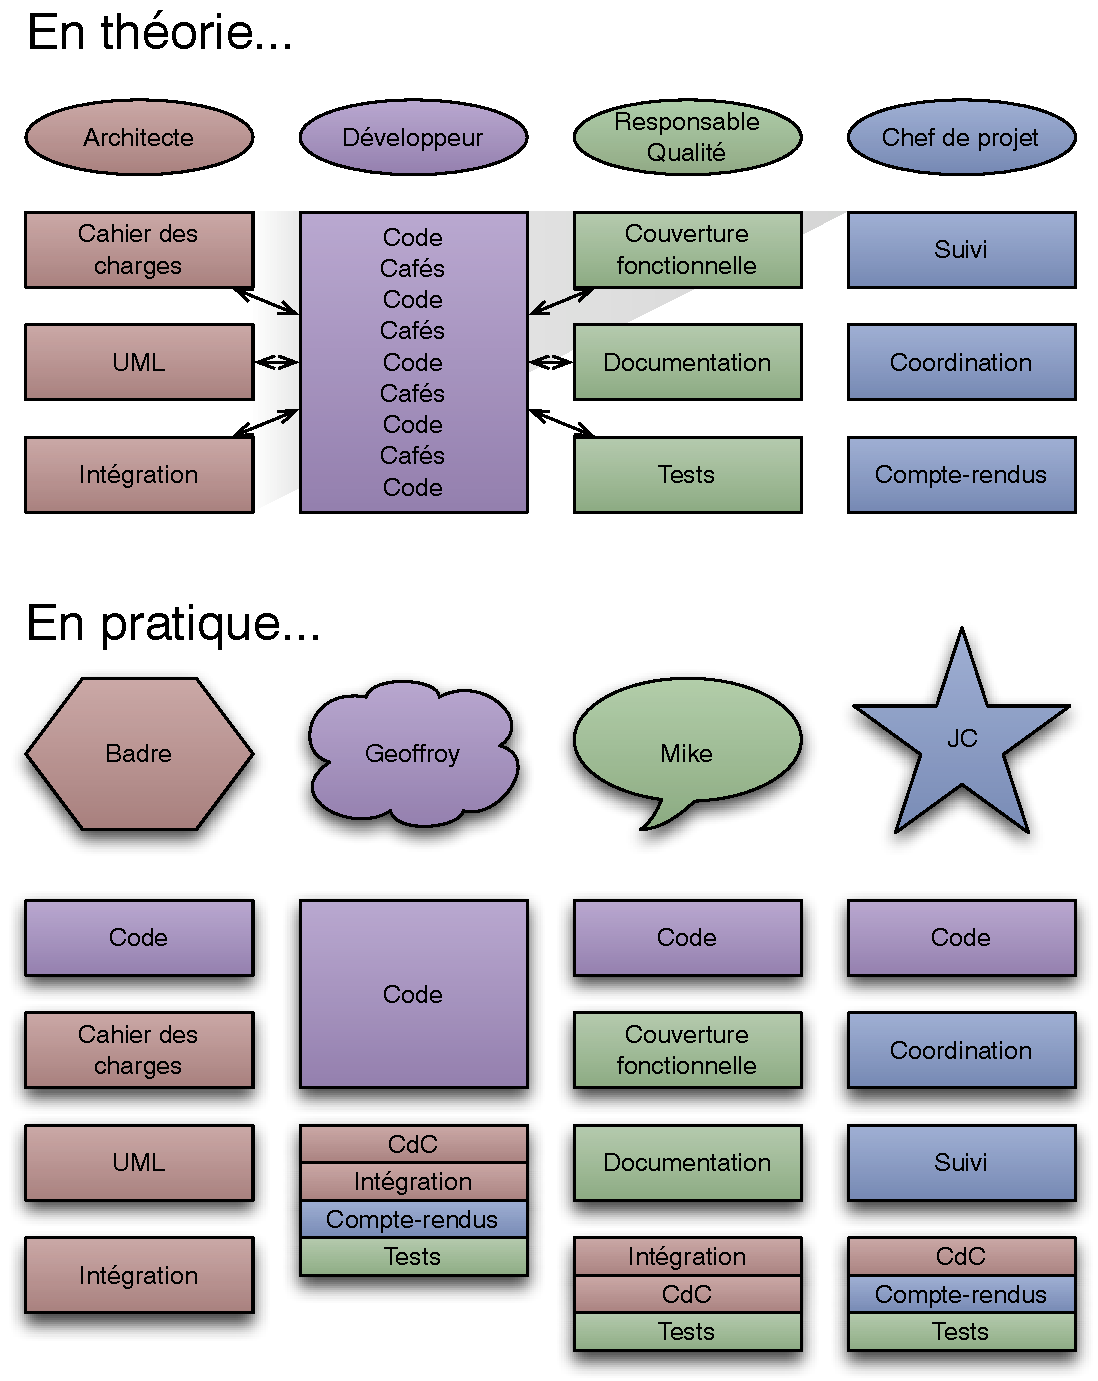
\includegraphics[width=20cm,angle=90]{../diagrammes/repartition_taches.pdf}
	\caption{Répartition des tâches}
	\label{fig:repartition}
\end{figure}

Nous avons répartis les tâches de chaque intervenant de notre équipe en adaptant les différentes responsabilité des postes attribués, tout en respectant les aspirations de chaque membre de l'équipe comme en témoigne la figure~\ref{fig:repartition},
p.~\pageref{fig:repartition}. Nous y présentons une structuration d'équipe par domaines de compétences, la répartition que nous prévoyons en début de projet et celle que nous avons observée.